\documentclass[twoside]{book}

% Packages required by doxygen
\usepackage{fixltx2e}
\usepackage{calc}
\usepackage{doxygen}
\usepackage[export]{adjustbox} % also loads graphicx
\usepackage{graphicx}
\usepackage[utf8]{inputenc}
\usepackage{makeidx}
\usepackage{multicol}
\usepackage{multirow}
\PassOptionsToPackage{warn}{textcomp}
\usepackage{textcomp}
\usepackage[nointegrals]{wasysym}
\usepackage[table]{xcolor}

% Font selection
\usepackage[T1]{fontenc}
\usepackage[scaled=.90]{helvet}
\usepackage{courier}
\usepackage{amssymb}
\usepackage{sectsty}
\renewcommand{\familydefault}{\sfdefault}
\allsectionsfont{%
  \fontseries{bc}\selectfont%
  \color{darkgray}%
}
\renewcommand{\DoxyLabelFont}{%
  \fontseries{bc}\selectfont%
  \color{darkgray}%
}
\newcommand{\+}{\discretionary{\mbox{\scriptsize$\hookleftarrow$}}{}{}}

% Page & text layout
\usepackage{geometry}
\geometry{%
  a4paper,%
  top=2.5cm,%
  bottom=2.5cm,%
  left=2.5cm,%
  right=2.5cm%
}
\tolerance=750
\hfuzz=15pt
\hbadness=750
\setlength{\emergencystretch}{15pt}
\setlength{\parindent}{0cm}
\setlength{\parskip}{3ex plus 2ex minus 2ex}
\makeatletter
\renewcommand{\paragraph}{%
  \@startsection{paragraph}{4}{0ex}{-1.0ex}{1.0ex}{%
    \normalfont\normalsize\bfseries\SS@parafont%
  }%
}
\renewcommand{\subparagraph}{%
  \@startsection{subparagraph}{5}{0ex}{-1.0ex}{1.0ex}{%
    \normalfont\normalsize\bfseries\SS@subparafont%
  }%
}
\makeatother

% Headers & footers
\usepackage{fancyhdr}
\pagestyle{fancyplain}
\fancyhead[LE]{\fancyplain{}{\bfseries\thepage}}
\fancyhead[CE]{\fancyplain{}{}}
\fancyhead[RE]{\fancyplain{}{\bfseries\leftmark}}
\fancyhead[LO]{\fancyplain{}{\bfseries\rightmark}}
\fancyhead[CO]{\fancyplain{}{}}
\fancyhead[RO]{\fancyplain{}{\bfseries\thepage}}
\fancyfoot[LE]{\fancyplain{}{}}
\fancyfoot[CE]{\fancyplain{}{}}
\fancyfoot[RE]{\fancyplain{}{\bfseries\scriptsize Generated by Doxygen }}
\fancyfoot[LO]{\fancyplain{}{\bfseries\scriptsize Generated by Doxygen }}
\fancyfoot[CO]{\fancyplain{}{}}
\fancyfoot[RO]{\fancyplain{}{}}
\renewcommand{\footrulewidth}{0.4pt}
\renewcommand{\chaptermark}[1]{%
  \markboth{#1}{}%
}
\renewcommand{\sectionmark}[1]{%
  \markright{\thesection\ #1}%
}

% Indices & bibliography
\usepackage{natbib}
\usepackage[titles]{tocloft}
\setcounter{tocdepth}{3}
\setcounter{secnumdepth}{5}
\makeindex

% Hyperlinks (required, but should be loaded last)
\usepackage{ifpdf}
\ifpdf
  \usepackage[pdftex,pagebackref=true]{hyperref}
\else
  \usepackage[ps2pdf,pagebackref=true]{hyperref}
\fi
\hypersetup{%
  colorlinks=true,%
  linkcolor=blue,%
  citecolor=blue,%
  unicode%
}

% Custom commands
\newcommand{\clearemptydoublepage}{%
  \newpage{\pagestyle{empty}\cleardoublepage}%
}

\usepackage{caption}
\captionsetup{labelsep=space,justification=centering,font={bf},singlelinecheck=off,skip=4pt,position=top}

%===== C O N T E N T S =====

\begin{document}

% Titlepage & ToC
\hypersetup{pageanchor=false,
             bookmarksnumbered=true,
             pdfencoding=unicode
            }
\pagenumbering{alph}
\begin{titlepage}
\vspace*{7cm}
\begin{center}%
{\Large C\+AD Software }\\
\vspace*{1cm}
{\large Generated by Doxygen 1.8.14}\\
\end{center}
\end{titlepage}
\clearemptydoublepage
\pagenumbering{roman}
\tableofcontents
\clearemptydoublepage
\pagenumbering{arabic}
\hypersetup{pageanchor=true}

%--- Begin generated contents ---
\chapter{q\+GL}
\label{md_src__r_e_a_d_m_e}
\Hypertarget{md_src__r_e_a_d_m_e}
\input{md_src__r_e_a_d_m_e}
\chapter{Hierarchical Index}
\section{Class Hierarchy}
This inheritance list is sorted roughly, but not completely, alphabetically\+:\begin{DoxyCompactList}
\item \contentsline{section}{Face}{\pageref{class_face}}{}
\item \contentsline{section}{Model}{\pageref{class_model}}{}
\item \contentsline{section}{Model2d}{\pageref{class_model2d}}{}
\item \contentsline{section}{Projection}{\pageref{class_projection}}{}
\item Q\+G\+L\+Widget\begin{DoxyCompactList}
\item \contentsline{section}{Glwidget}{\pageref{class_glwidget}}{}
\item \contentsline{section}{ProjectionX}{\pageref{class_projection_x}}{}
\item \contentsline{section}{ProjectionY}{\pageref{class_projection_y}}{}
\item \contentsline{section}{ProjectionZ}{\pageref{class_projection_z}}{}
\end{DoxyCompactList}
\item Q\+Main\+Window\begin{DoxyCompactList}
\item \contentsline{section}{Main\+Window}{\pageref{class_main_window}}{}
\end{DoxyCompactList}
\item \contentsline{section}{Sample\+Models}{\pageref{class_sample_models}}{}
\end{DoxyCompactList}

\chapter{Class Index}
\section{Class List}
Here are the classes, structs, unions and interfaces with brief descriptions\+:\begin{DoxyCompactList}
\item\contentsline{section}{\mbox{\hyperlink{class_face}{Face}} \\*Holds objects that are used to describe the faces in rendering the 3d model using open\+GL }{\pageref{class_face}}{}
\item\contentsline{section}{\mbox{\hyperlink{class_glwidget}{Glwidget}} }{\pageref{class_glwidget}}{}
\item\contentsline{section}{\mbox{\hyperlink{class_main_window}{Main\+Window}} }{\pageref{class_main_window}}{}
\item\contentsline{section}{\mbox{\hyperlink{class_model}{Model}} }{\pageref{class_model}}{}
\item\contentsline{section}{\mbox{\hyperlink{class_model2d}{Model2d}} \\*Creates the 2d model for a particular design by defining the necessary attributes }{\pageref{class_model2d}}{}
\item\contentsline{section}{\mbox{\hyperlink{class_projection}{Projection}} }{\pageref{class_projection}}{}
\item\contentsline{section}{\mbox{\hyperlink{class_projection_x}{ProjectionX}} \\*Defines the projectionX for the current design to be displayed using the model class }{\pageref{class_projection_x}}{}
\item\contentsline{section}{\mbox{\hyperlink{class_projection_y}{ProjectionY}} \\*Defines the projectionY for the current design to be displayed using the model class }{\pageref{class_projection_y}}{}
\item\contentsline{section}{\mbox{\hyperlink{class_projection_z}{ProjectionZ}} \\*Defines the projectionZ for the current design to be displayed using the model class }{\pageref{class_projection_z}}{}
\item\contentsline{section}{\mbox{\hyperlink{class_sample_models}{Sample\+Models}} \\*Defines the templates for the software including other necessary designs for base display like the axes }{\pageref{class_sample_models}}{}
\end{DoxyCompactList}

\chapter{Class Documentation}
\hypertarget{class_face}{}\section{Face Class Reference}
\label{class_face}\index{Face@{Face}}


Collaboration diagram for Face\+:
\nopagebreak
\begin{figure}[H]
\begin{center}
\leavevmode
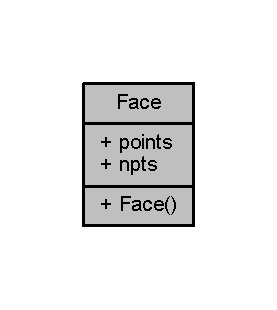
\includegraphics[width=133pt]{class_face__coll__graph}
\end{center}
\end{figure}
\subsection*{Public Member Functions}
\begin{DoxyCompactItemize}
\item 
\mbox{\Hypertarget{class_face_a890f52c15855e434e6c0f853bcf7f40d}\label{class_face_a890f52c15855e434e6c0f853bcf7f40d}} 
{\bfseries Face} (float $\ast$pts, int npts)
\end{DoxyCompactItemize}
\subsection*{Public Attributes}
\begin{DoxyCompactItemize}
\item 
\mbox{\Hypertarget{class_face_a402240ad45f918a772d83f3022f9589f}\label{class_face_a402240ad45f918a772d83f3022f9589f}} 
float $\ast$ {\bfseries points}
\item 
\mbox{\Hypertarget{class_face_ac35360914de7ce1903058a598b9fe7ab}\label{class_face_ac35360914de7ce1903058a598b9fe7ab}} 
int {\bfseries npts}
\end{DoxyCompactItemize}


The documentation for this class was generated from the following files\+:\begin{DoxyCompactItemize}
\item 
src/model.\+h\item 
src/model.\+cpp\end{DoxyCompactItemize}

\hypertarget{class_glwidget}{}\section{Glwidget Class Reference}
\label{class_glwidget}\index{Glwidget@{Glwidget}}


{\ttfamily \#include $<$glwidget.\+h$>$}



Inheritance diagram for Glwidget\+:\nopagebreak
\begin{figure}[H]
\begin{center}
\leavevmode
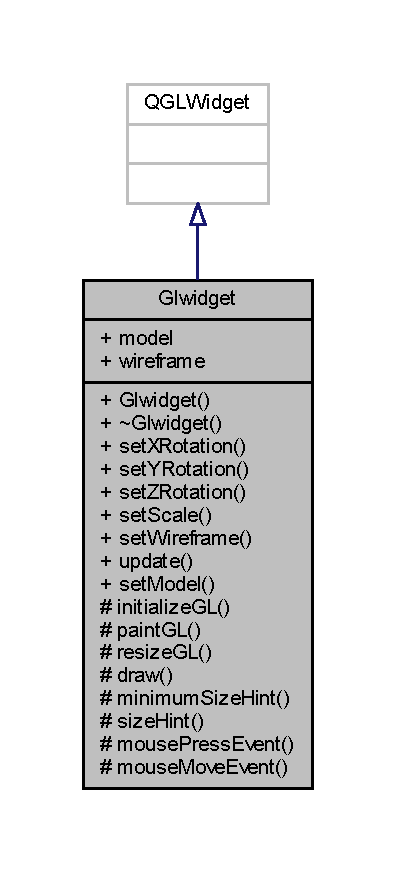
\includegraphics[width=190pt]{class_glwidget__inherit__graph}
\end{center}
\end{figure}


Collaboration diagram for Glwidget\+:\nopagebreak
\begin{figure}[H]
\begin{center}
\leavevmode
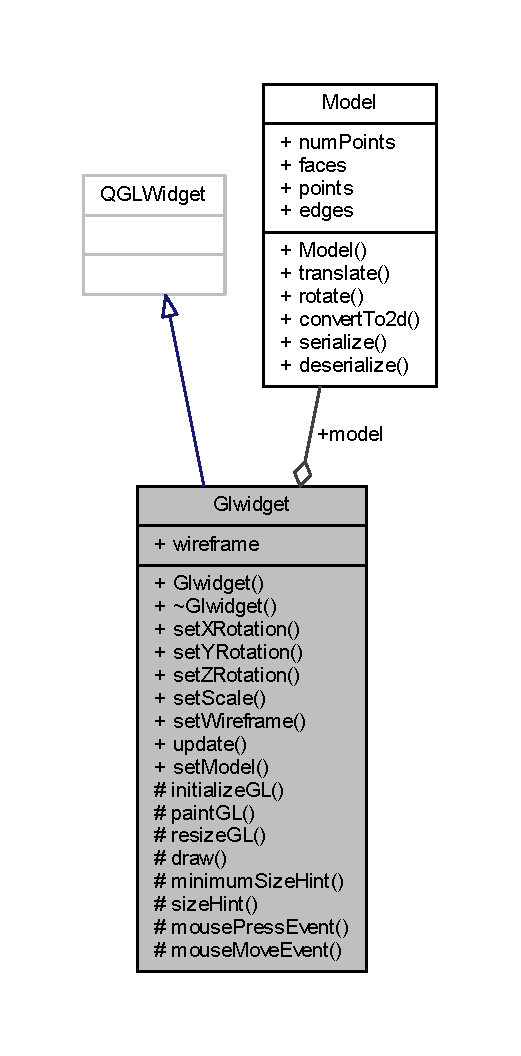
\includegraphics[width=250pt]{class_glwidget__coll__graph}
\end{center}
\end{figure}
\subsection*{Public Slots}
\begin{DoxyCompactItemize}
\item 
void \mbox{\hyperlink{class_glwidget_abdb807d1e98041d3813543dd2f043d9e}{set\+X\+Rotation}} (int angle)
\item 
void \mbox{\hyperlink{class_glwidget_a980d52bca9bf5817911029877a68e584}{set\+Y\+Rotation}} (int angle)
\item 
void \mbox{\hyperlink{class_glwidget_ad9318fc18c0abc761ce038c6afbf1814}{set\+Z\+Rotation}} (int angle)
\item 
void \mbox{\hyperlink{class_glwidget_a2ea79df264aadd3584488296749f370c}{set\+Scale}} (int factor)
\item 
void \mbox{\hyperlink{class_glwidget_a52a956313956890bf13741c218f8fa3d}{set\+Wireframe}} (bool b)
\item 
void \mbox{\hyperlink{class_glwidget_a2b49ec71ab84e52adc78ba062c235ac0}{update}} ()
\item 
void \mbox{\hyperlink{class_glwidget_a2786dcfd2ee92efbbd2c457dc1ac7063}{set\+Model}} (\mbox{\hyperlink{class_model}{Model}} $\ast$m)
\end{DoxyCompactItemize}
\subsection*{Signals}
\begin{DoxyCompactItemize}
\item 
void \mbox{\hyperlink{class_glwidget_a179006a4c52b573f9e6791deb16f1f2a}{x\+Rotation\+Changed}} (int angle)
\item 
void \mbox{\hyperlink{class_glwidget_a7c8d9abf4c47760ea6c6fff8ed12e0a5}{y\+Rotation\+Changed}} (int angle)
\item 
void \mbox{\hyperlink{class_glwidget_ab1b7ea4daa9671708ba4dd12fa8c52a9}{z\+Rotation\+Changed}} (int angle)
\item 
void \mbox{\hyperlink{class_glwidget_a874d1da9fed05d5063176ec5195aa483}{scale\+Changed}} (int factor)
\end{DoxyCompactItemize}
\subsection*{Public Member Functions}
\begin{DoxyCompactItemize}
\item 
\mbox{\hyperlink{class_glwidget_a498977aa216afadd4adba780063356ac}{Glwidget}} (Q\+Widget $\ast$parent=0)
\item 
\mbox{\hyperlink{class_glwidget_acaef15b194db8b00381aaa0e7e4c9389}{$\sim$\+Glwidget}} ()
\end{DoxyCompactItemize}
\subsection*{Public Attributes}
\begin{DoxyCompactItemize}
\item 
\mbox{\hyperlink{class_model}{Model}} $\ast$ \mbox{\hyperlink{class_glwidget_a160da762ff1b4a6c1bf6f09bfb71e15c}{model}}
\item 
bool \mbox{\hyperlink{class_glwidget_abe8b6e5adc693200d652414fd8929f46}{wireframe}}
\end{DoxyCompactItemize}
\subsection*{Protected Member Functions}
\begin{DoxyCompactItemize}
\item 
void \mbox{\hyperlink{class_glwidget_a5f266609dcd89e1291539a498ce42cbb}{initialize\+GL}} ()
\item 
void \mbox{\hyperlink{class_glwidget_a440fe507a9bd647c1a961cf72305da31}{paint\+GL}} ()
\item 
void \mbox{\hyperlink{class_glwidget_a36bd98ea1696cf1a7f5830fde3a16a72}{resize\+GL}} (int width, int height)
\item 
void \mbox{\hyperlink{class_glwidget_ac54d1b859e11037f3e86f3193e84970b}{draw}} ()
\item 
Q\+Size \mbox{\hyperlink{class_glwidget_a9768cbeb06b6ccfaff47ff443dda1c98}{minimum\+Size\+Hint}} () const
\item 
Q\+Size \mbox{\hyperlink{class_glwidget_a0dfc5b597184e106d7bcf921ba24b09a}{size\+Hint}} () const
\item 
void \mbox{\hyperlink{class_glwidget_a0e3f033e0fa941505114a32d35823c70}{mouse\+Press\+Event}} (Q\+Mouse\+Event $\ast$event)
\item 
void \mbox{\hyperlink{class_glwidget_afc8a6da76c5ead92b1c1a4ba8f931310}{mouse\+Move\+Event}} (Q\+Mouse\+Event $\ast$event)
\end{DoxyCompactItemize}


\subsection{Constructor \& Destructor Documentation}
\mbox{\Hypertarget{class_glwidget_a498977aa216afadd4adba780063356ac}\label{class_glwidget_a498977aa216afadd4adba780063356ac}} 
\index{Glwidget@{Glwidget}!Glwidget@{Glwidget}}
\index{Glwidget@{Glwidget}!Glwidget@{Glwidget}}
\subsubsection{\texorpdfstring{Glwidget()}{Glwidget()}}
{\footnotesize\ttfamily Glwidget\+::\+Glwidget (\begin{DoxyParamCaption}\item[{Q\+Widget $\ast$}]{parent = {\ttfamily 0} }\end{DoxyParamCaption})\hspace{0.3cm}{\ttfamily [explicit]}}

\mbox{\Hypertarget{class_glwidget_acaef15b194db8b00381aaa0e7e4c9389}\label{class_glwidget_acaef15b194db8b00381aaa0e7e4c9389}} 
\index{Glwidget@{Glwidget}!````~Glwidget@{$\sim$\+Glwidget}}
\index{````~Glwidget@{$\sim$\+Glwidget}!Glwidget@{Glwidget}}
\subsubsection{\texorpdfstring{$\sim$\+Glwidget()}{~Glwidget()}}
{\footnotesize\ttfamily Glwidget\+::$\sim$\+Glwidget (\begin{DoxyParamCaption}{ }\end{DoxyParamCaption})}



\subsection{Member Function Documentation}
\mbox{\Hypertarget{class_glwidget_ac54d1b859e11037f3e86f3193e84970b}\label{class_glwidget_ac54d1b859e11037f3e86f3193e84970b}} 
\index{Glwidget@{Glwidget}!draw@{draw}}
\index{draw@{draw}!Glwidget@{Glwidget}}
\subsubsection{\texorpdfstring{draw()}{draw()}}
{\footnotesize\ttfamily void Glwidget\+::draw (\begin{DoxyParamCaption}{ }\end{DoxyParamCaption})\hspace{0.3cm}{\ttfamily [protected]}}

\mbox{\Hypertarget{class_glwidget_a5f266609dcd89e1291539a498ce42cbb}\label{class_glwidget_a5f266609dcd89e1291539a498ce42cbb}} 
\index{Glwidget@{Glwidget}!initialize\+GL@{initialize\+GL}}
\index{initialize\+GL@{initialize\+GL}!Glwidget@{Glwidget}}
\subsubsection{\texorpdfstring{initialize\+G\+L()}{initializeGL()}}
{\footnotesize\ttfamily void Glwidget\+::initialize\+GL (\begin{DoxyParamCaption}{ }\end{DoxyParamCaption})\hspace{0.3cm}{\ttfamily [protected]}}

\mbox{\Hypertarget{class_glwidget_a9768cbeb06b6ccfaff47ff443dda1c98}\label{class_glwidget_a9768cbeb06b6ccfaff47ff443dda1c98}} 
\index{Glwidget@{Glwidget}!minimum\+Size\+Hint@{minimum\+Size\+Hint}}
\index{minimum\+Size\+Hint@{minimum\+Size\+Hint}!Glwidget@{Glwidget}}
\subsubsection{\texorpdfstring{minimum\+Size\+Hint()}{minimumSizeHint()}}
{\footnotesize\ttfamily Q\+Size Glwidget\+::minimum\+Size\+Hint (\begin{DoxyParamCaption}{ }\end{DoxyParamCaption}) const\hspace{0.3cm}{\ttfamily [protected]}}

\mbox{\Hypertarget{class_glwidget_afc8a6da76c5ead92b1c1a4ba8f931310}\label{class_glwidget_afc8a6da76c5ead92b1c1a4ba8f931310}} 
\index{Glwidget@{Glwidget}!mouse\+Move\+Event@{mouse\+Move\+Event}}
\index{mouse\+Move\+Event@{mouse\+Move\+Event}!Glwidget@{Glwidget}}
\subsubsection{\texorpdfstring{mouse\+Move\+Event()}{mouseMoveEvent()}}
{\footnotesize\ttfamily void Glwidget\+::mouse\+Move\+Event (\begin{DoxyParamCaption}\item[{Q\+Mouse\+Event $\ast$}]{event }\end{DoxyParamCaption})\hspace{0.3cm}{\ttfamily [protected]}}

\mbox{\Hypertarget{class_glwidget_a0e3f033e0fa941505114a32d35823c70}\label{class_glwidget_a0e3f033e0fa941505114a32d35823c70}} 
\index{Glwidget@{Glwidget}!mouse\+Press\+Event@{mouse\+Press\+Event}}
\index{mouse\+Press\+Event@{mouse\+Press\+Event}!Glwidget@{Glwidget}}
\subsubsection{\texorpdfstring{mouse\+Press\+Event()}{mousePressEvent()}}
{\footnotesize\ttfamily void Glwidget\+::mouse\+Press\+Event (\begin{DoxyParamCaption}\item[{Q\+Mouse\+Event $\ast$}]{event }\end{DoxyParamCaption})\hspace{0.3cm}{\ttfamily [protected]}}

\mbox{\Hypertarget{class_glwidget_a440fe507a9bd647c1a961cf72305da31}\label{class_glwidget_a440fe507a9bd647c1a961cf72305da31}} 
\index{Glwidget@{Glwidget}!paint\+GL@{paint\+GL}}
\index{paint\+GL@{paint\+GL}!Glwidget@{Glwidget}}
\subsubsection{\texorpdfstring{paint\+G\+L()}{paintGL()}}
{\footnotesize\ttfamily void Glwidget\+::paint\+GL (\begin{DoxyParamCaption}{ }\end{DoxyParamCaption})\hspace{0.3cm}{\ttfamily [protected]}}

\mbox{\Hypertarget{class_glwidget_a36bd98ea1696cf1a7f5830fde3a16a72}\label{class_glwidget_a36bd98ea1696cf1a7f5830fde3a16a72}} 
\index{Glwidget@{Glwidget}!resize\+GL@{resize\+GL}}
\index{resize\+GL@{resize\+GL}!Glwidget@{Glwidget}}
\subsubsection{\texorpdfstring{resize\+G\+L()}{resizeGL()}}
{\footnotesize\ttfamily void Glwidget\+::resize\+GL (\begin{DoxyParamCaption}\item[{int}]{width,  }\item[{int}]{height }\end{DoxyParamCaption})\hspace{0.3cm}{\ttfamily [protected]}}

\mbox{\Hypertarget{class_glwidget_a874d1da9fed05d5063176ec5195aa483}\label{class_glwidget_a874d1da9fed05d5063176ec5195aa483}} 
\index{Glwidget@{Glwidget}!scale\+Changed@{scale\+Changed}}
\index{scale\+Changed@{scale\+Changed}!Glwidget@{Glwidget}}
\subsubsection{\texorpdfstring{scale\+Changed}{scaleChanged}}
{\footnotesize\ttfamily void Glwidget\+::scale\+Changed (\begin{DoxyParamCaption}\item[{int}]{factor }\end{DoxyParamCaption})\hspace{0.3cm}{\ttfamily [signal]}}

\mbox{\Hypertarget{class_glwidget_a2786dcfd2ee92efbbd2c457dc1ac7063}\label{class_glwidget_a2786dcfd2ee92efbbd2c457dc1ac7063}} 
\index{Glwidget@{Glwidget}!set\+Model@{set\+Model}}
\index{set\+Model@{set\+Model}!Glwidget@{Glwidget}}
\subsubsection{\texorpdfstring{set\+Model}{setModel}}
{\footnotesize\ttfamily void Glwidget\+::set\+Model (\begin{DoxyParamCaption}\item[{\mbox{\hyperlink{class_model}{Model}} $\ast$}]{m }\end{DoxyParamCaption})\hspace{0.3cm}{\ttfamily [slot]}}

\mbox{\Hypertarget{class_glwidget_a2ea79df264aadd3584488296749f370c}\label{class_glwidget_a2ea79df264aadd3584488296749f370c}} 
\index{Glwidget@{Glwidget}!set\+Scale@{set\+Scale}}
\index{set\+Scale@{set\+Scale}!Glwidget@{Glwidget}}
\subsubsection{\texorpdfstring{set\+Scale}{setScale}}
{\footnotesize\ttfamily void Glwidget\+::set\+Scale (\begin{DoxyParamCaption}\item[{int}]{factor }\end{DoxyParamCaption})\hspace{0.3cm}{\ttfamily [slot]}}

\mbox{\Hypertarget{class_glwidget_a52a956313956890bf13741c218f8fa3d}\label{class_glwidget_a52a956313956890bf13741c218f8fa3d}} 
\index{Glwidget@{Glwidget}!set\+Wireframe@{set\+Wireframe}}
\index{set\+Wireframe@{set\+Wireframe}!Glwidget@{Glwidget}}
\subsubsection{\texorpdfstring{set\+Wireframe}{setWireframe}}
{\footnotesize\ttfamily void Glwidget\+::set\+Wireframe (\begin{DoxyParamCaption}\item[{bool}]{b }\end{DoxyParamCaption})\hspace{0.3cm}{\ttfamily [slot]}}

\mbox{\Hypertarget{class_glwidget_abdb807d1e98041d3813543dd2f043d9e}\label{class_glwidget_abdb807d1e98041d3813543dd2f043d9e}} 
\index{Glwidget@{Glwidget}!set\+X\+Rotation@{set\+X\+Rotation}}
\index{set\+X\+Rotation@{set\+X\+Rotation}!Glwidget@{Glwidget}}
\subsubsection{\texorpdfstring{set\+X\+Rotation}{setXRotation}}
{\footnotesize\ttfamily void Glwidget\+::set\+X\+Rotation (\begin{DoxyParamCaption}\item[{int}]{angle }\end{DoxyParamCaption})\hspace{0.3cm}{\ttfamily [slot]}}

\mbox{\Hypertarget{class_glwidget_a980d52bca9bf5817911029877a68e584}\label{class_glwidget_a980d52bca9bf5817911029877a68e584}} 
\index{Glwidget@{Glwidget}!set\+Y\+Rotation@{set\+Y\+Rotation}}
\index{set\+Y\+Rotation@{set\+Y\+Rotation}!Glwidget@{Glwidget}}
\subsubsection{\texorpdfstring{set\+Y\+Rotation}{setYRotation}}
{\footnotesize\ttfamily void Glwidget\+::set\+Y\+Rotation (\begin{DoxyParamCaption}\item[{int}]{angle }\end{DoxyParamCaption})\hspace{0.3cm}{\ttfamily [slot]}}

\mbox{\Hypertarget{class_glwidget_ad9318fc18c0abc761ce038c6afbf1814}\label{class_glwidget_ad9318fc18c0abc761ce038c6afbf1814}} 
\index{Glwidget@{Glwidget}!set\+Z\+Rotation@{set\+Z\+Rotation}}
\index{set\+Z\+Rotation@{set\+Z\+Rotation}!Glwidget@{Glwidget}}
\subsubsection{\texorpdfstring{set\+Z\+Rotation}{setZRotation}}
{\footnotesize\ttfamily void Glwidget\+::set\+Z\+Rotation (\begin{DoxyParamCaption}\item[{int}]{angle }\end{DoxyParamCaption})\hspace{0.3cm}{\ttfamily [slot]}}

\mbox{\Hypertarget{class_glwidget_a0dfc5b597184e106d7bcf921ba24b09a}\label{class_glwidget_a0dfc5b597184e106d7bcf921ba24b09a}} 
\index{Glwidget@{Glwidget}!size\+Hint@{size\+Hint}}
\index{size\+Hint@{size\+Hint}!Glwidget@{Glwidget}}
\subsubsection{\texorpdfstring{size\+Hint()}{sizeHint()}}
{\footnotesize\ttfamily Q\+Size Glwidget\+::size\+Hint (\begin{DoxyParamCaption}{ }\end{DoxyParamCaption}) const\hspace{0.3cm}{\ttfamily [protected]}}

\mbox{\Hypertarget{class_glwidget_a2b49ec71ab84e52adc78ba062c235ac0}\label{class_glwidget_a2b49ec71ab84e52adc78ba062c235ac0}} 
\index{Glwidget@{Glwidget}!update@{update}}
\index{update@{update}!Glwidget@{Glwidget}}
\subsubsection{\texorpdfstring{update}{update}}
{\footnotesize\ttfamily void Glwidget\+::update (\begin{DoxyParamCaption}{ }\end{DoxyParamCaption})\hspace{0.3cm}{\ttfamily [slot]}}

\mbox{\Hypertarget{class_glwidget_a179006a4c52b573f9e6791deb16f1f2a}\label{class_glwidget_a179006a4c52b573f9e6791deb16f1f2a}} 
\index{Glwidget@{Glwidget}!x\+Rotation\+Changed@{x\+Rotation\+Changed}}
\index{x\+Rotation\+Changed@{x\+Rotation\+Changed}!Glwidget@{Glwidget}}
\subsubsection{\texorpdfstring{x\+Rotation\+Changed}{xRotationChanged}}
{\footnotesize\ttfamily void Glwidget\+::x\+Rotation\+Changed (\begin{DoxyParamCaption}\item[{int}]{angle }\end{DoxyParamCaption})\hspace{0.3cm}{\ttfamily [signal]}}

\mbox{\Hypertarget{class_glwidget_a7c8d9abf4c47760ea6c6fff8ed12e0a5}\label{class_glwidget_a7c8d9abf4c47760ea6c6fff8ed12e0a5}} 
\index{Glwidget@{Glwidget}!y\+Rotation\+Changed@{y\+Rotation\+Changed}}
\index{y\+Rotation\+Changed@{y\+Rotation\+Changed}!Glwidget@{Glwidget}}
\subsubsection{\texorpdfstring{y\+Rotation\+Changed}{yRotationChanged}}
{\footnotesize\ttfamily void Glwidget\+::y\+Rotation\+Changed (\begin{DoxyParamCaption}\item[{int}]{angle }\end{DoxyParamCaption})\hspace{0.3cm}{\ttfamily [signal]}}

\mbox{\Hypertarget{class_glwidget_ab1b7ea4daa9671708ba4dd12fa8c52a9}\label{class_glwidget_ab1b7ea4daa9671708ba4dd12fa8c52a9}} 
\index{Glwidget@{Glwidget}!z\+Rotation\+Changed@{z\+Rotation\+Changed}}
\index{z\+Rotation\+Changed@{z\+Rotation\+Changed}!Glwidget@{Glwidget}}
\subsubsection{\texorpdfstring{z\+Rotation\+Changed}{zRotationChanged}}
{\footnotesize\ttfamily void Glwidget\+::z\+Rotation\+Changed (\begin{DoxyParamCaption}\item[{int}]{angle }\end{DoxyParamCaption})\hspace{0.3cm}{\ttfamily [signal]}}



\subsection{Member Data Documentation}
\mbox{\Hypertarget{class_glwidget_a160da762ff1b4a6c1bf6f09bfb71e15c}\label{class_glwidget_a160da762ff1b4a6c1bf6f09bfb71e15c}} 
\index{Glwidget@{Glwidget}!model@{model}}
\index{model@{model}!Glwidget@{Glwidget}}
\subsubsection{\texorpdfstring{model}{model}}
{\footnotesize\ttfamily \mbox{\hyperlink{class_model}{Model}}$\ast$ Glwidget\+::model}

\mbox{\Hypertarget{class_glwidget_abe8b6e5adc693200d652414fd8929f46}\label{class_glwidget_abe8b6e5adc693200d652414fd8929f46}} 
\index{Glwidget@{Glwidget}!wireframe@{wireframe}}
\index{wireframe@{wireframe}!Glwidget@{Glwidget}}
\subsubsection{\texorpdfstring{wireframe}{wireframe}}
{\footnotesize\ttfamily bool Glwidget\+::wireframe}



The documentation for this class was generated from the following files\+:\begin{DoxyCompactItemize}
\item 
src/\mbox{\hyperlink{glwidget_8h}{glwidget.\+h}}\item 
src/\mbox{\hyperlink{glwidget_8cpp}{glwidget.\+cpp}}\end{DoxyCompactItemize}

\hypertarget{class_main_window}{}\section{Main\+Window Class Reference}
\label{class_main_window}\index{Main\+Window@{Main\+Window}}


Inheritance diagram for Main\+Window\+:
\nopagebreak
\begin{figure}[H]
\begin{center}
\leavevmode
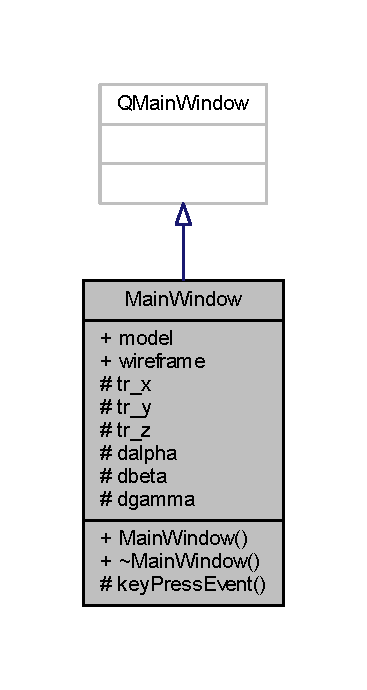
\includegraphics[width=176pt]{class_main_window__inherit__graph}
\end{center}
\end{figure}


Collaboration diagram for Main\+Window\+:
\nopagebreak
\begin{figure}[H]
\begin{center}
\leavevmode
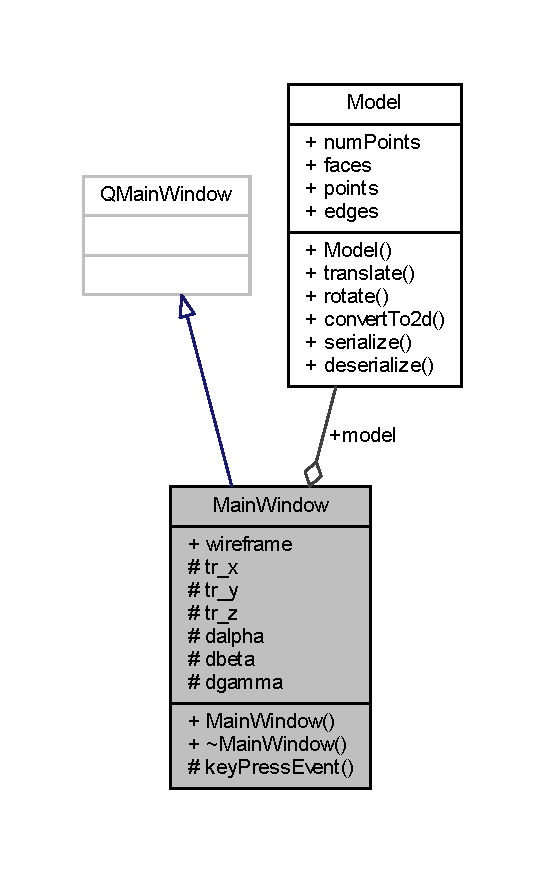
\includegraphics[width=262pt]{class_main_window__coll__graph}
\end{center}
\end{figure}
\subsection*{Signals}
\begin{DoxyCompactItemize}
\item 
\mbox{\Hypertarget{class_main_window_a482b2d965f153134f11f834fcd28fed5}\label{class_main_window_a482b2d965f153134f11f834fcd28fed5}} 
void {\bfseries wireframe\+Val} (bool b)
\item 
\mbox{\Hypertarget{class_main_window_a9bd4c07ced537631f1e93c8b5888e78d}\label{class_main_window_a9bd4c07ced537631f1e93c8b5888e78d}} 
void {\bfseries get\+Model} (\mbox{\hyperlink{class_model}{Model}} $\ast$m)
\item 
\mbox{\Hypertarget{class_main_window_a128f71880d4b9683149023fc46fcc9f8}\label{class_main_window_a128f71880d4b9683149023fc46fcc9f8}} 
void {\bfseries update} ()
\end{DoxyCompactItemize}
\subsection*{Public Member Functions}
\begin{DoxyCompactItemize}
\item 
\mbox{\Hypertarget{class_main_window_a8b244be8b7b7db1b08de2a2acb9409db}\label{class_main_window_a8b244be8b7b7db1b08de2a2acb9409db}} 
{\bfseries Main\+Window} (Q\+Widget $\ast$parent=0)
\end{DoxyCompactItemize}
\subsection*{Public Attributes}
\begin{DoxyCompactItemize}
\item 
\mbox{\Hypertarget{class_main_window_a6ceb394c6a471fb60dce6bd3f7c78475}\label{class_main_window_a6ceb394c6a471fb60dce6bd3f7c78475}} 
\mbox{\hyperlink{class_model}{Model}} $\ast$ {\bfseries model}
\item 
\mbox{\Hypertarget{class_main_window_aa63776c884a82936064be5aabe3da6e8}\label{class_main_window_aa63776c884a82936064be5aabe3da6e8}} 
bool {\bfseries wireframe}
\end{DoxyCompactItemize}
\subsection*{Protected Member Functions}
\begin{DoxyCompactItemize}
\item 
\mbox{\Hypertarget{class_main_window_a9c4f542263838b9ecd06eae839a42a34}\label{class_main_window_a9c4f542263838b9ecd06eae839a42a34}} 
void {\bfseries key\+Press\+Event} (Q\+Key\+Event $\ast$event)
\end{DoxyCompactItemize}
\subsection*{Protected Attributes}
\begin{DoxyCompactItemize}
\item 
\mbox{\Hypertarget{class_main_window_a243e9877c34fca99ca8eb8233e602e80}\label{class_main_window_a243e9877c34fca99ca8eb8233e602e80}} 
float {\bfseries tr\+\_\+x}
\item 
\mbox{\Hypertarget{class_main_window_a93fc2a7aa546e29b1ec00c81d278d9c2}\label{class_main_window_a93fc2a7aa546e29b1ec00c81d278d9c2}} 
float {\bfseries tr\+\_\+y}
\item 
\mbox{\Hypertarget{class_main_window_a48e1e4cfdaa4d52f32b46ece5e1e785b}\label{class_main_window_a48e1e4cfdaa4d52f32b46ece5e1e785b}} 
float {\bfseries tr\+\_\+z}
\item 
\mbox{\Hypertarget{class_main_window_a8a40d17a32ac50fc54faf17a3ddc1b21}\label{class_main_window_a8a40d17a32ac50fc54faf17a3ddc1b21}} 
float {\bfseries dalpha}
\item 
\mbox{\Hypertarget{class_main_window_a7a6b42f86582dd883162c70d4a4915c8}\label{class_main_window_a7a6b42f86582dd883162c70d4a4915c8}} 
float {\bfseries dbeta}
\item 
\mbox{\Hypertarget{class_main_window_ac10de49b138c1c838d53e12da4c24d6d}\label{class_main_window_ac10de49b138c1c838d53e12da4c24d6d}} 
float {\bfseries dgamma}
\end{DoxyCompactItemize}


The documentation for this class was generated from the following files\+:\begin{DoxyCompactItemize}
\item 
src/mainwindow.\+h\item 
src/mainwindow.\+cpp\end{DoxyCompactItemize}

\hypertarget{class_model}{}\section{Model Class Reference}
\label{class_model}\index{Model@{Model}}


{\ttfamily \#include $<$model.\+h$>$}



Collaboration diagram for Model\+:\nopagebreak
\begin{figure}[H]
\begin{center}
\leavevmode
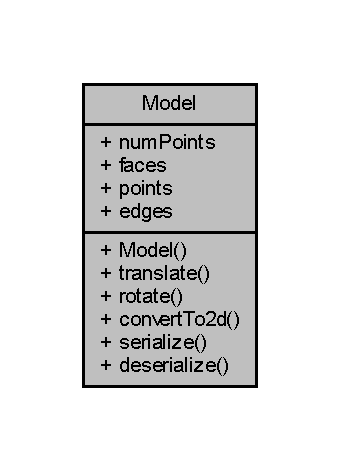
\includegraphics[width=163pt]{class_model__coll__graph}
\end{center}
\end{figure}
\subsection*{Public Member Functions}
\begin{DoxyCompactItemize}
\item 
\mbox{\hyperlink{class_model_a39cf79e51da0f52f1031f98f1bebd118}{Model}} (int \mbox{\hyperlink{class_model_a39ac6e91375d5ac5799a9845c3479d9c}{num\+Points}}, float $\ast$pts, bool $\ast$$\ast$\mbox{\hyperlink{class_model_a723a0c631c2ff688fed06c5652879ef7}{edges}}, std\+::vector$<$ \mbox{\hyperlink{class_face}{Face}} $\ast$$>$ \mbox{\hyperlink{class_model_a7752ae8e1bbacc53ed94d7bd9c404b6d}{faces}})
\begin{DoxyCompactList}\small\item\em Constructor for the 3d model. \end{DoxyCompactList}\item 
void \mbox{\hyperlink{class_model_a32e61c8487a2202e9f3f041a8abcb3c2}{translate}} (float dx, float dy, float dz)
\begin{DoxyCompactList}\small\item\em translates the model by the specified values along the respective directions \end{DoxyCompactList}\item 
void \mbox{\hyperlink{class_model_ae5999fb77646320aed8d81a669568caa}{rotate}} (float alpha, float beta, float gamma)
\begin{DoxyCompactList}\small\item\em rotates the object with respect to the axes by the specifies angles along x,y,z axes respectively \end{DoxyCompactList}\item 
\mbox{\hyperlink{class_model2d}{Model2d}} $\ast$ \mbox{\hyperlink{class_model_ac62fb1874a6597955c89fe3a9a1663e1}{convert\+To2d}} ()
\begin{DoxyCompactList}\small\item\em generates the 2d model object for the current 3d model \end{DoxyCompactList}\item 
void \mbox{\hyperlink{class_model_abc71b3488f7f944f1c99727a491ee985}{serialize}} (std\+::string s)
\begin{DoxyCompactList}\small\item\em used to generate the text that specifies the 3d model to be saved in a text file \end{DoxyCompactList}\end{DoxyCompactItemize}
\subsection*{Static Public Member Functions}
\begin{DoxyCompactItemize}
\item 
static \mbox{\hyperlink{class_model}{Model}} $\ast$ \mbox{\hyperlink{class_model_a98946d1c8d49b43f541dbd6b98b31e52}{deserialize}} (std\+::string s)
\begin{DoxyCompactList}\small\item\em used to generate the 3d model from the text code saved in a particular file \end{DoxyCompactList}\end{DoxyCompactItemize}
\subsection*{Public Attributes}
\begin{DoxyCompactItemize}
\item 
int \mbox{\hyperlink{class_model_a39ac6e91375d5ac5799a9845c3479d9c}{num\+Points}}
\begin{DoxyCompactList}\small\item\em the number of vertices that describe the model \end{DoxyCompactList}\item 
std\+::vector$<$ \mbox{\hyperlink{class_face}{Face}} $\ast$ $>$ \mbox{\hyperlink{class_model_a7752ae8e1bbacc53ed94d7bd9c404b6d}{faces}}
\begin{DoxyCompactList}\small\item\em the vector containing the faces that describes the 3d model \end{DoxyCompactList}\item 
float $\ast$ \mbox{\hyperlink{class_model_a6436acbcf42bece5621666fe37c71309}{points}}
\begin{DoxyCompactList}\small\item\em the array of points in 3d \end{DoxyCompactList}\item 
bool $\ast$$\ast$ \mbox{\hyperlink{class_model_a723a0c631c2ff688fed06c5652879ef7}{edges}}
\begin{DoxyCompactList}\small\item\em the double array of the edges between the vertices of the model described by a bool value \end{DoxyCompactList}\end{DoxyCompactItemize}


\subsection{Constructor \& Destructor Documentation}
\mbox{\Hypertarget{class_model_a39cf79e51da0f52f1031f98f1bebd118}\label{class_model_a39cf79e51da0f52f1031f98f1bebd118}} 
\index{Model@{Model}!Model@{Model}}
\index{Model@{Model}!Model@{Model}}
\subsubsection{\texorpdfstring{Model()}{Model()}}
{\footnotesize\ttfamily Model\+::\+Model (\begin{DoxyParamCaption}\item[{int}]{num\+Points,  }\item[{float $\ast$}]{pts,  }\item[{bool $\ast$$\ast$}]{edges,  }\item[{std\+::vector$<$ \mbox{\hyperlink{class_face}{Face}} $\ast$$>$}]{faces }\end{DoxyParamCaption})}



Constructor for the 3d model. 



\subsection{Member Function Documentation}
\mbox{\Hypertarget{class_model_ac62fb1874a6597955c89fe3a9a1663e1}\label{class_model_ac62fb1874a6597955c89fe3a9a1663e1}} 
\index{Model@{Model}!convert\+To2d@{convert\+To2d}}
\index{convert\+To2d@{convert\+To2d}!Model@{Model}}
\subsubsection{\texorpdfstring{convert\+To2d()}{convertTo2d()}}
{\footnotesize\ttfamily \mbox{\hyperlink{class_model2d}{Model2d}} $\ast$ Model\+::convert\+To2d (\begin{DoxyParamCaption}{ }\end{DoxyParamCaption})}



generates the 2d model object for the current 3d model 

\mbox{\Hypertarget{class_model_a98946d1c8d49b43f541dbd6b98b31e52}\label{class_model_a98946d1c8d49b43f541dbd6b98b31e52}} 
\index{Model@{Model}!deserialize@{deserialize}}
\index{deserialize@{deserialize}!Model@{Model}}
\subsubsection{\texorpdfstring{deserialize()}{deserialize()}}
{\footnotesize\ttfamily \mbox{\hyperlink{class_model}{Model}} $\ast$ Model\+::deserialize (\begin{DoxyParamCaption}\item[{std\+::string}]{s }\end{DoxyParamCaption})\hspace{0.3cm}{\ttfamily [static]}}



used to generate the 3d model from the text code saved in a particular file 

\mbox{\Hypertarget{class_model_ae5999fb77646320aed8d81a669568caa}\label{class_model_ae5999fb77646320aed8d81a669568caa}} 
\index{Model@{Model}!rotate@{rotate}}
\index{rotate@{rotate}!Model@{Model}}
\subsubsection{\texorpdfstring{rotate()}{rotate()}}
{\footnotesize\ttfamily void Model\+::rotate (\begin{DoxyParamCaption}\item[{float}]{alpha,  }\item[{float}]{beta,  }\item[{float}]{gamma }\end{DoxyParamCaption})}



rotates the object with respect to the axes by the specifies angles along x,y,z axes respectively 

\mbox{\Hypertarget{class_model_abc71b3488f7f944f1c99727a491ee985}\label{class_model_abc71b3488f7f944f1c99727a491ee985}} 
\index{Model@{Model}!serialize@{serialize}}
\index{serialize@{serialize}!Model@{Model}}
\subsubsection{\texorpdfstring{serialize()}{serialize()}}
{\footnotesize\ttfamily void Model\+::serialize (\begin{DoxyParamCaption}\item[{std\+::string}]{s }\end{DoxyParamCaption})}



used to generate the text that specifies the 3d model to be saved in a text file 

\mbox{\Hypertarget{class_model_a32e61c8487a2202e9f3f041a8abcb3c2}\label{class_model_a32e61c8487a2202e9f3f041a8abcb3c2}} 
\index{Model@{Model}!translate@{translate}}
\index{translate@{translate}!Model@{Model}}
\subsubsection{\texorpdfstring{translate()}{translate()}}
{\footnotesize\ttfamily void Model\+::translate (\begin{DoxyParamCaption}\item[{float}]{dx,  }\item[{float}]{dy,  }\item[{float}]{dz }\end{DoxyParamCaption})}



translates the model by the specified values along the respective directions 



\subsection{Member Data Documentation}
\mbox{\Hypertarget{class_model_a723a0c631c2ff688fed06c5652879ef7}\label{class_model_a723a0c631c2ff688fed06c5652879ef7}} 
\index{Model@{Model}!edges@{edges}}
\index{edges@{edges}!Model@{Model}}
\subsubsection{\texorpdfstring{edges}{edges}}
{\footnotesize\ttfamily bool$\ast$$\ast$ Model\+::edges}



the double array of the edges between the vertices of the model described by a bool value 

\mbox{\Hypertarget{class_model_a7752ae8e1bbacc53ed94d7bd9c404b6d}\label{class_model_a7752ae8e1bbacc53ed94d7bd9c404b6d}} 
\index{Model@{Model}!faces@{faces}}
\index{faces@{faces}!Model@{Model}}
\subsubsection{\texorpdfstring{faces}{faces}}
{\footnotesize\ttfamily std\+::vector$<$\mbox{\hyperlink{class_face}{Face}}$\ast$$>$ Model\+::faces}



the vector containing the faces that describes the 3d model 

\mbox{\Hypertarget{class_model_a39ac6e91375d5ac5799a9845c3479d9c}\label{class_model_a39ac6e91375d5ac5799a9845c3479d9c}} 
\index{Model@{Model}!num\+Points@{num\+Points}}
\index{num\+Points@{num\+Points}!Model@{Model}}
\subsubsection{\texorpdfstring{num\+Points}{numPoints}}
{\footnotesize\ttfamily int Model\+::num\+Points}



the number of vertices that describe the model 

\mbox{\Hypertarget{class_model_a6436acbcf42bece5621666fe37c71309}\label{class_model_a6436acbcf42bece5621666fe37c71309}} 
\index{Model@{Model}!points@{points}}
\index{points@{points}!Model@{Model}}
\subsubsection{\texorpdfstring{points}{points}}
{\footnotesize\ttfamily float$\ast$ Model\+::points}



the array of points in 3d 



The documentation for this class was generated from the following files\+:\begin{DoxyCompactItemize}
\item 
src/\mbox{\hyperlink{model_8h}{model.\+h}}\item 
src/\mbox{\hyperlink{model_8cpp}{model.\+cpp}}\end{DoxyCompactItemize}

\hypertarget{class_model2d}{}\section{Model2d Class Reference}
\label{class_model2d}\index{Model2d@{Model2d}}


Collaboration diagram for Model2d\+:
\nopagebreak
\begin{figure}[H]
\begin{center}
\leavevmode
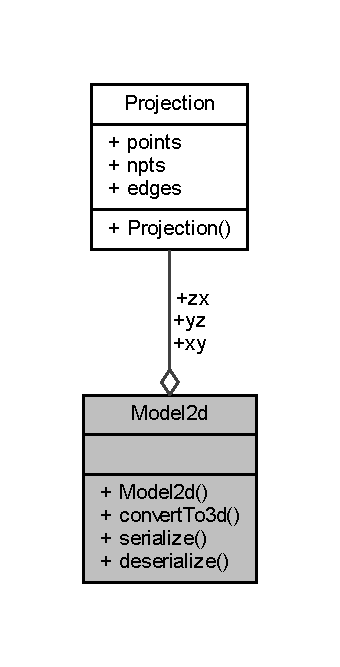
\includegraphics[width=163pt]{class_model2d__coll__graph}
\end{center}
\end{figure}
\subsection*{Public Member Functions}
\begin{DoxyCompactItemize}
\item 
\mbox{\Hypertarget{class_model2d_aa07204b20301739146f8ecf525778720}\label{class_model2d_aa07204b20301739146f8ecf525778720}} 
{\bfseries Model2d} (\mbox{\hyperlink{class_projection}{Projection}} $\ast$xy, \mbox{\hyperlink{class_projection}{Projection}} $\ast$yz, \mbox{\hyperlink{class_projection}{Projection}} $\ast$zx)
\item 
\mbox{\Hypertarget{class_model2d_ab39a4f4a2c6430cee2b226a9509ec38b}\label{class_model2d_ab39a4f4a2c6430cee2b226a9509ec38b}} 
\mbox{\hyperlink{class_model}{Model}} $\ast$ {\bfseries convert\+To3d} ()
\item 
\mbox{\Hypertarget{class_model2d_a9dbe9eafd94b347c3257ac90e743065c}\label{class_model2d_a9dbe9eafd94b347c3257ac90e743065c}} 
void {\bfseries serialize} (std\+::string s)
\end{DoxyCompactItemize}
\subsection*{Static Public Member Functions}
\begin{DoxyCompactItemize}
\item 
\mbox{\Hypertarget{class_model2d_aa3c8399ef5cf86bb176b111c132f30b7}\label{class_model2d_aa3c8399ef5cf86bb176b111c132f30b7}} 
static \mbox{\hyperlink{class_model2d}{Model2d}} $\ast$ {\bfseries deserialize} (std\+::string s)
\end{DoxyCompactItemize}
\subsection*{Public Attributes}
\begin{DoxyCompactItemize}
\item 
\mbox{\Hypertarget{class_model2d_ad335c0d9899b23996a3f11e61be1d431}\label{class_model2d_ad335c0d9899b23996a3f11e61be1d431}} 
\mbox{\hyperlink{class_projection}{Projection}} $\ast$ {\bfseries xy}
\item 
\mbox{\Hypertarget{class_model2d_a4d012de876b8bb089bd226e41270df25}\label{class_model2d_a4d012de876b8bb089bd226e41270df25}} 
\mbox{\hyperlink{class_projection}{Projection}} $\ast$ {\bfseries yz}
\item 
\mbox{\Hypertarget{class_model2d_a6c459c26e4c89bbc11ac0149ea07b997}\label{class_model2d_a6c459c26e4c89bbc11ac0149ea07b997}} 
\mbox{\hyperlink{class_projection}{Projection}} $\ast$ {\bfseries zx}
\end{DoxyCompactItemize}


The documentation for this class was generated from the following files\+:\begin{DoxyCompactItemize}
\item 
src/model2d.\+h\item 
src/model2d.\+cpp\end{DoxyCompactItemize}

\hypertarget{class_projection}{}\section{Projection Class Reference}
\label{class_projection}\index{Projection@{Projection}}


Collaboration diagram for Projection\+:
\nopagebreak
\begin{figure}[H]
\begin{center}
\leavevmode
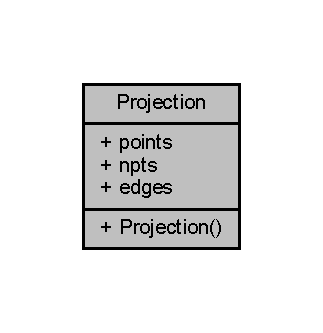
\includegraphics[width=155pt]{class_projection__coll__graph}
\end{center}
\end{figure}
\subsection*{Public Member Functions}
\begin{DoxyCompactItemize}
\item 
\mbox{\Hypertarget{class_projection_a5308ac2fb97e9805c76e3cf767f08a0e}\label{class_projection_a5308ac2fb97e9805c76e3cf767f08a0e}} 
{\bfseries Projection} (int num\+Points, float $\ast$points, bool $\ast$$\ast$edges)
\end{DoxyCompactItemize}
\subsection*{Public Attributes}
\begin{DoxyCompactItemize}
\item 
\mbox{\Hypertarget{class_projection_aa42ba5494690dbfa5f875472adc97789}\label{class_projection_aa42ba5494690dbfa5f875472adc97789}} 
float $\ast$ {\bfseries points}
\item 
\mbox{\Hypertarget{class_projection_a6972ab0bc1cfa26a5480a940d66e3497}\label{class_projection_a6972ab0bc1cfa26a5480a940d66e3497}} 
int {\bfseries npts}
\item 
\mbox{\Hypertarget{class_projection_a7943c696e88d15825dee0641b269b5f7}\label{class_projection_a7943c696e88d15825dee0641b269b5f7}} 
bool $\ast$$\ast$ {\bfseries edges}
\end{DoxyCompactItemize}


The documentation for this class was generated from the following files\+:\begin{DoxyCompactItemize}
\item 
src/model2d.\+h\item 
src/model2d.\+cpp\end{DoxyCompactItemize}

\hypertarget{class_projection_x}{}\section{ProjectionX Class Reference}
\label{class_projection_x}\index{ProjectionX@{ProjectionX}}


Inheritance diagram for ProjectionX\+:
\nopagebreak
\begin{figure}[H]
\begin{center}
\leavevmode
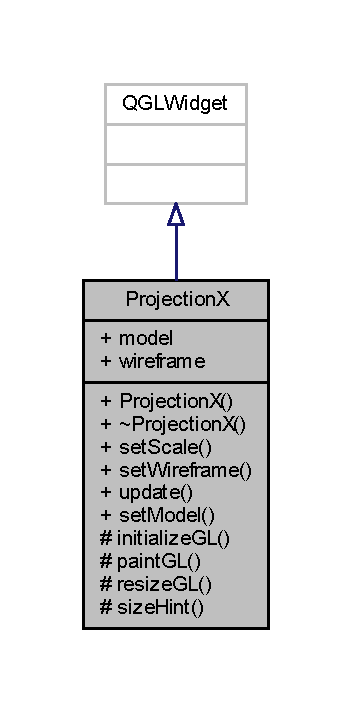
\includegraphics[width=169pt]{class_projection_x__inherit__graph}
\end{center}
\end{figure}


Collaboration diagram for ProjectionX\+:
\nopagebreak
\begin{figure}[H]
\begin{center}
\leavevmode
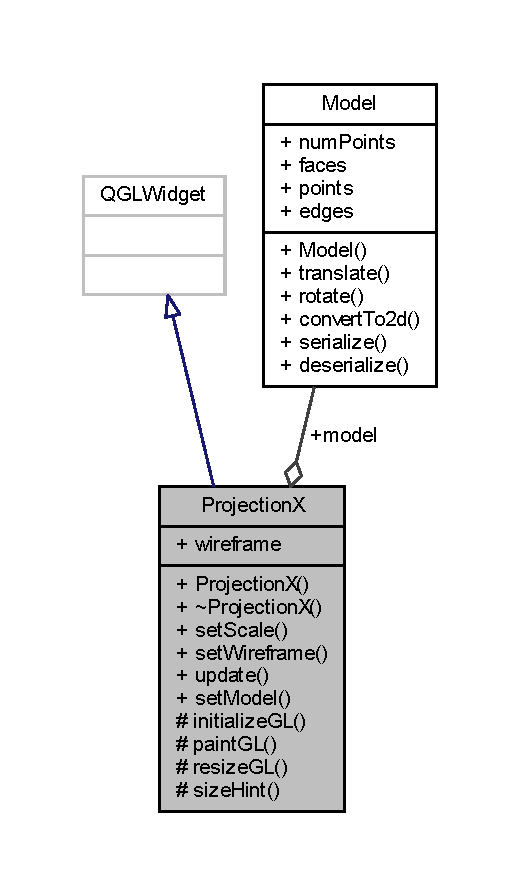
\includegraphics[width=250pt]{class_projection_x__coll__graph}
\end{center}
\end{figure}
\subsection*{Public Slots}
\begin{DoxyCompactItemize}
\item 
\mbox{\Hypertarget{class_projection_x_a863c01fcbb77cb13856feb3605fc6390}\label{class_projection_x_a863c01fcbb77cb13856feb3605fc6390}} 
void {\bfseries set\+Scale} (int factor)
\item 
\mbox{\Hypertarget{class_projection_x_a16849f2ef9fe0332c0ad9f833dc85651}\label{class_projection_x_a16849f2ef9fe0332c0ad9f833dc85651}} 
void {\bfseries set\+Wireframe} (bool b)
\item 
\mbox{\Hypertarget{class_projection_x_a7efa3839fdf999686464fe60ea59a349}\label{class_projection_x_a7efa3839fdf999686464fe60ea59a349}} 
void {\bfseries update} ()
\item 
\mbox{\Hypertarget{class_projection_x_aab00d67a74912bdff9f963664b708c14}\label{class_projection_x_aab00d67a74912bdff9f963664b708c14}} 
void {\bfseries set\+Model} (\mbox{\hyperlink{class_model}{Model}} $\ast$m)
\end{DoxyCompactItemize}
\subsection*{Public Member Functions}
\begin{DoxyCompactItemize}
\item 
\mbox{\Hypertarget{class_projection_x_a251536fb76aabbf276ce0cd2341d1dc3}\label{class_projection_x_a251536fb76aabbf276ce0cd2341d1dc3}} 
{\bfseries ProjectionX} (Q\+Widget $\ast$parent=0)
\end{DoxyCompactItemize}
\subsection*{Public Attributes}
\begin{DoxyCompactItemize}
\item 
\mbox{\Hypertarget{class_projection_x_af85d1d33a1a51fa6aef5359f53b98580}\label{class_projection_x_af85d1d33a1a51fa6aef5359f53b98580}} 
\mbox{\hyperlink{class_model}{Model}} $\ast$ {\bfseries model}
\item 
\mbox{\Hypertarget{class_projection_x_aa9a1f3880a2084eb87cbbe0f98c67a64}\label{class_projection_x_aa9a1f3880a2084eb87cbbe0f98c67a64}} 
bool {\bfseries wireframe}
\end{DoxyCompactItemize}
\subsection*{Protected Member Functions}
\begin{DoxyCompactItemize}
\item 
\mbox{\Hypertarget{class_projection_x_af94caa374ed76c3cf81c80429c67aee9}\label{class_projection_x_af94caa374ed76c3cf81c80429c67aee9}} 
void {\bfseries initialize\+GL} ()
\item 
\mbox{\Hypertarget{class_projection_x_a4fff0844542e49a68b0288c85703b1c4}\label{class_projection_x_a4fff0844542e49a68b0288c85703b1c4}} 
void {\bfseries paint\+GL} ()
\item 
\mbox{\Hypertarget{class_projection_x_a7eb1ba9a4266f65982357e53142bc693}\label{class_projection_x_a7eb1ba9a4266f65982357e53142bc693}} 
void {\bfseries resize\+GL} (int width, int height)
\item 
\mbox{\Hypertarget{class_projection_x_ad1a6cdc49e0cb1000bc67401a6a8b3a9}\label{class_projection_x_ad1a6cdc49e0cb1000bc67401a6a8b3a9}} 
Q\+Size {\bfseries size\+Hint} () const
\end{DoxyCompactItemize}


The documentation for this class was generated from the following files\+:\begin{DoxyCompactItemize}
\item 
src/projectionx.\+h\item 
src/projectionx.\+cpp\end{DoxyCompactItemize}

\hypertarget{class_projection_y}{}\section{ProjectionY Class Reference}
\label{class_projection_y}\index{ProjectionY@{ProjectionY}}


Inheritance diagram for ProjectionY\+:
\nopagebreak
\begin{figure}[H]
\begin{center}
\leavevmode
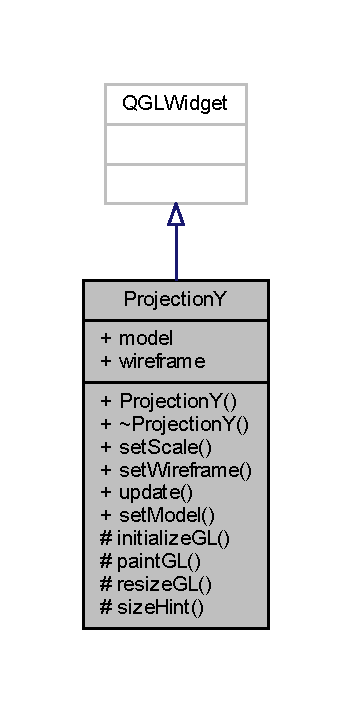
\includegraphics[width=169pt]{class_projection_y__inherit__graph}
\end{center}
\end{figure}


Collaboration diagram for ProjectionY\+:
\nopagebreak
\begin{figure}[H]
\begin{center}
\leavevmode
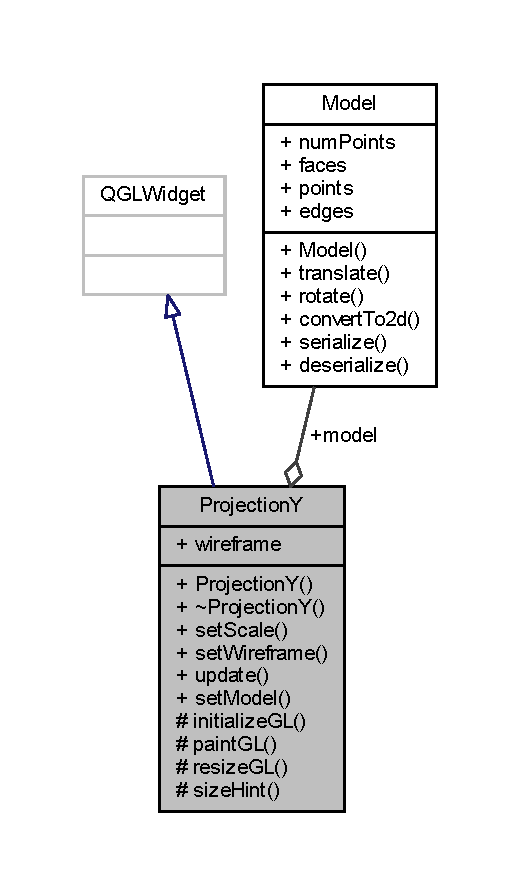
\includegraphics[width=250pt]{class_projection_y__coll__graph}
\end{center}
\end{figure}
\subsection*{Public Slots}
\begin{DoxyCompactItemize}
\item 
\mbox{\Hypertarget{class_projection_y_a19960a2d4075443ab87fd50147fee276}\label{class_projection_y_a19960a2d4075443ab87fd50147fee276}} 
void {\bfseries set\+Scale} (int factor)
\item 
\mbox{\Hypertarget{class_projection_y_ab59d0f6245e889c25faf1d0592145d6c}\label{class_projection_y_ab59d0f6245e889c25faf1d0592145d6c}} 
void {\bfseries set\+Wireframe} (bool b)
\item 
\mbox{\Hypertarget{class_projection_y_a3c709da38e36be432cdc3979cf37d527}\label{class_projection_y_a3c709da38e36be432cdc3979cf37d527}} 
void {\bfseries update} ()
\item 
\mbox{\Hypertarget{class_projection_y_a66e7b460c9bb0c02b649a241d3b9a647}\label{class_projection_y_a66e7b460c9bb0c02b649a241d3b9a647}} 
void {\bfseries set\+Model} (\mbox{\hyperlink{class_model}{Model}} $\ast$m)
\end{DoxyCompactItemize}
\subsection*{Public Member Functions}
\begin{DoxyCompactItemize}
\item 
\mbox{\Hypertarget{class_projection_y_ada83942857907322b5bad855f34ee893}\label{class_projection_y_ada83942857907322b5bad855f34ee893}} 
{\bfseries ProjectionY} (Q\+Widget $\ast$parent=0)
\end{DoxyCompactItemize}
\subsection*{Public Attributes}
\begin{DoxyCompactItemize}
\item 
\mbox{\Hypertarget{class_projection_y_a5fef5122782e5ed50e7dd2f302628852}\label{class_projection_y_a5fef5122782e5ed50e7dd2f302628852}} 
\mbox{\hyperlink{class_model}{Model}} $\ast$ {\bfseries model}
\item 
\mbox{\Hypertarget{class_projection_y_a8ac9c3d56c5dd9ca94afee7bfe4526d1}\label{class_projection_y_a8ac9c3d56c5dd9ca94afee7bfe4526d1}} 
bool {\bfseries wireframe}
\end{DoxyCompactItemize}
\subsection*{Protected Member Functions}
\begin{DoxyCompactItemize}
\item 
\mbox{\Hypertarget{class_projection_y_aa241c90c6d57dedc345ce447de8b2062}\label{class_projection_y_aa241c90c6d57dedc345ce447de8b2062}} 
void {\bfseries initialize\+GL} ()
\item 
\mbox{\Hypertarget{class_projection_y_ad71d2f89a6b30e2979d5cfe2af2a4128}\label{class_projection_y_ad71d2f89a6b30e2979d5cfe2af2a4128}} 
void {\bfseries paint\+GL} ()
\item 
\mbox{\Hypertarget{class_projection_y_a0e2001d9ee85afa0ce1ad8b2b8f15ad7}\label{class_projection_y_a0e2001d9ee85afa0ce1ad8b2b8f15ad7}} 
void {\bfseries resize\+GL} (int width, int height)
\item 
\mbox{\Hypertarget{class_projection_y_a8d502c7b1fc7cb5c894a84f10fba7368}\label{class_projection_y_a8d502c7b1fc7cb5c894a84f10fba7368}} 
Q\+Size {\bfseries size\+Hint} () const
\end{DoxyCompactItemize}


The documentation for this class was generated from the following files\+:\begin{DoxyCompactItemize}
\item 
src/projectiony.\+h\item 
src/projectiony.\+cpp\end{DoxyCompactItemize}

\hypertarget{class_projection_z}{}\section{ProjectionZ Class Reference}
\label{class_projection_z}\index{ProjectionZ@{ProjectionZ}}


defines the projectionZ for the current design to be displayed using the model class  




{\ttfamily \#include $<$projectionz.\+h$>$}



Inheritance diagram for ProjectionZ\+:\nopagebreak
\begin{figure}[H]
\begin{center}
\leavevmode
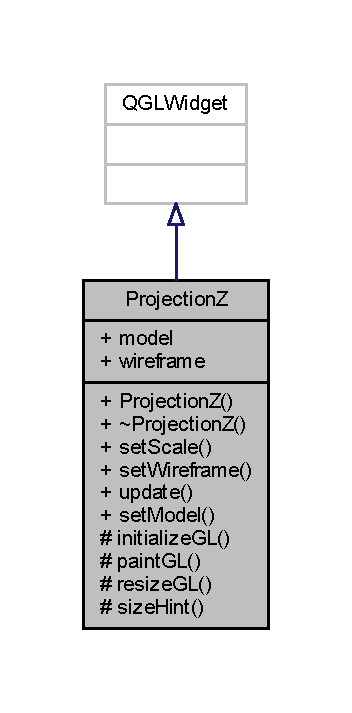
\includegraphics[width=169pt]{class_projection_z__inherit__graph}
\end{center}
\end{figure}


Collaboration diagram for ProjectionZ\+:\nopagebreak
\begin{figure}[H]
\begin{center}
\leavevmode
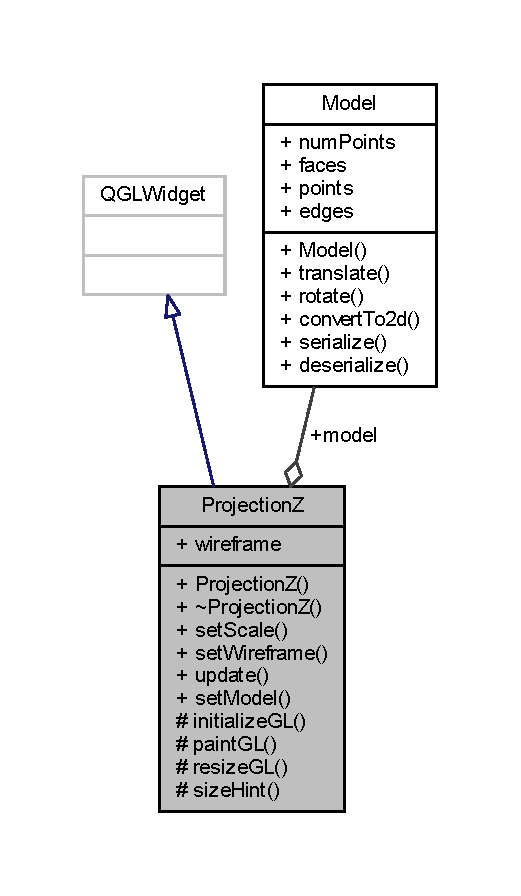
\includegraphics[width=250pt]{class_projection_z__coll__graph}
\end{center}
\end{figure}
\subsection*{Public Slots}
\begin{DoxyCompactItemize}
\item 
void \mbox{\hyperlink{class_projection_z_a21e56fe128f64983203888507845847d}{set\+Scale}} (int factor)
\begin{DoxyCompactList}\small\item\em decide the numerical scale factor for viewing the object \end{DoxyCompactList}\item 
void \mbox{\hyperlink{class_projection_z_a61a7115d258f9324b5f697983dd5ca3d}{set\+Wireframe}} (bool b)
\begin{DoxyCompactList}\small\item\em set the wrireframe property of the model \end{DoxyCompactList}\item 
void \mbox{\hyperlink{class_projection_z_abf7cbd3b5479c7805fbceecf3c68b0be}{update}} ()
\begin{DoxyCompactList}\small\item\em the update function just updates the model view based on its currently set parameters/fields \end{DoxyCompactList}\item 
void \mbox{\hyperlink{class_projection_z_af65afd9bf93b40bbf626cd2fba303b3f}{set\+Model}} (\mbox{\hyperlink{class_model}{Model}} $\ast$m)
\begin{DoxyCompactList}\small\item\em sets the current model to the specified argument \end{DoxyCompactList}\end{DoxyCompactItemize}
\subsection*{Public Member Functions}
\begin{DoxyCompactItemize}
\item 
\mbox{\hyperlink{class_projection_z_ac812d46606329365a4e877b6cc58d86d}{ProjectionZ}} (Q\+Widget $\ast$parent=0)
\item 
\mbox{\hyperlink{class_projection_z_a5d1f4701bf63635f88924761f26ce173}{$\sim$\+ProjectionZ}} ()
\end{DoxyCompactItemize}
\subsection*{Public Attributes}
\begin{DoxyCompactItemize}
\item 
\mbox{\hyperlink{class_model}{Model}} $\ast$ \mbox{\hyperlink{class_projection_z_a72def73a612bcd05243ae8acad447908}{model}}
\begin{DoxyCompactList}\small\item\em the 3d model that describes a xy projection view \end{DoxyCompactList}\item 
bool \mbox{\hyperlink{class_projection_z_a24466982ce2e792bb843426c35782222}{wireframe}}
\begin{DoxyCompactList}\small\item\em the wireframe is either enabled or disabled for the projection \end{DoxyCompactList}\end{DoxyCompactItemize}
\subsection*{Protected Member Functions}
\begin{DoxyCompactItemize}
\item 
void \mbox{\hyperlink{class_projection_z_aa470131d521e6595d293e12f0fa3425f}{initialize\+GL}} ()
\begin{DoxyCompactList}\small\item\em sets up the Open\+GL resources and state. Gets called once before the first time \mbox{\hyperlink{class_projection_z_a5f276e00f3680aa3ec663030e74df160}{resize\+G\+L()}} or \mbox{\hyperlink{class_projection_z_a192e7a4a75e41e9d2c411eb252c2d2d6}{paint\+G\+L()}} is called \end{DoxyCompactList}\item 
void \mbox{\hyperlink{class_projection_z_a192e7a4a75e41e9d2c411eb252c2d2d6}{paint\+GL}} ()
\begin{DoxyCompactList}\small\item\em renders the Open\+GL scene. Gets called whenever the widget needs to be updated \end{DoxyCompactList}\item 
void \mbox{\hyperlink{class_projection_z_a5f276e00f3680aa3ec663030e74df160}{resize\+GL}} (int width, int height)
\begin{DoxyCompactList}\small\item\em sets up the Open\+GL viewport, projection, etc. Gets called whenever the widget has been resized (and also when it is shown for the first time because all newly created widgets get a resize event automatically). \end{DoxyCompactList}\item 
Q\+Size \mbox{\hyperlink{class_projection_z_a5baf9e15d828cff9501fd94fa622b32b}{size\+Hint}} () const
\begin{DoxyCompactList}\small\item\em to provide a reasonable default size for the widget \end{DoxyCompactList}\end{DoxyCompactItemize}


\subsection{Detailed Description}
defines the projectionZ for the current design to be displayed using the model class 

\subsection{Constructor \& Destructor Documentation}
\mbox{\Hypertarget{class_projection_z_ac812d46606329365a4e877b6cc58d86d}\label{class_projection_z_ac812d46606329365a4e877b6cc58d86d}} 
\index{ProjectionZ@{ProjectionZ}!ProjectionZ@{ProjectionZ}}
\index{ProjectionZ@{ProjectionZ}!ProjectionZ@{ProjectionZ}}
\subsubsection{\texorpdfstring{Projection\+Z()}{ProjectionZ()}}
{\footnotesize\ttfamily Projection\+Z\+::\+ProjectionZ (\begin{DoxyParamCaption}\item[{Q\+Widget $\ast$}]{parent = {\ttfamily 0} }\end{DoxyParamCaption})\hspace{0.3cm}{\ttfamily [explicit]}}

\mbox{\Hypertarget{class_projection_z_a5d1f4701bf63635f88924761f26ce173}\label{class_projection_z_a5d1f4701bf63635f88924761f26ce173}} 
\index{ProjectionZ@{ProjectionZ}!````~ProjectionZ@{$\sim$\+ProjectionZ}}
\index{````~ProjectionZ@{$\sim$\+ProjectionZ}!ProjectionZ@{ProjectionZ}}
\subsubsection{\texorpdfstring{$\sim$\+Projection\+Z()}{~ProjectionZ()}}
{\footnotesize\ttfamily Projection\+Z\+::$\sim$\+ProjectionZ (\begin{DoxyParamCaption}{ }\end{DoxyParamCaption})}



\subsection{Member Function Documentation}
\mbox{\Hypertarget{class_projection_z_aa470131d521e6595d293e12f0fa3425f}\label{class_projection_z_aa470131d521e6595d293e12f0fa3425f}} 
\index{ProjectionZ@{ProjectionZ}!initialize\+GL@{initialize\+GL}}
\index{initialize\+GL@{initialize\+GL}!ProjectionZ@{ProjectionZ}}
\subsubsection{\texorpdfstring{initialize\+G\+L()}{initializeGL()}}
{\footnotesize\ttfamily void Projection\+Z\+::initialize\+GL (\begin{DoxyParamCaption}{ }\end{DoxyParamCaption})\hspace{0.3cm}{\ttfamily [protected]}}



sets up the Open\+GL resources and state. Gets called once before the first time \mbox{\hyperlink{class_projection_z_a5f276e00f3680aa3ec663030e74df160}{resize\+G\+L()}} or \mbox{\hyperlink{class_projection_z_a192e7a4a75e41e9d2c411eb252c2d2d6}{paint\+G\+L()}} is called 

\mbox{\Hypertarget{class_projection_z_a192e7a4a75e41e9d2c411eb252c2d2d6}\label{class_projection_z_a192e7a4a75e41e9d2c411eb252c2d2d6}} 
\index{ProjectionZ@{ProjectionZ}!paint\+GL@{paint\+GL}}
\index{paint\+GL@{paint\+GL}!ProjectionZ@{ProjectionZ}}
\subsubsection{\texorpdfstring{paint\+G\+L()}{paintGL()}}
{\footnotesize\ttfamily void Projection\+Z\+::paint\+GL (\begin{DoxyParamCaption}{ }\end{DoxyParamCaption})\hspace{0.3cm}{\ttfamily [protected]}}



renders the Open\+GL scene. Gets called whenever the widget needs to be updated 

\mbox{\Hypertarget{class_projection_z_a5f276e00f3680aa3ec663030e74df160}\label{class_projection_z_a5f276e00f3680aa3ec663030e74df160}} 
\index{ProjectionZ@{ProjectionZ}!resize\+GL@{resize\+GL}}
\index{resize\+GL@{resize\+GL}!ProjectionZ@{ProjectionZ}}
\subsubsection{\texorpdfstring{resize\+G\+L()}{resizeGL()}}
{\footnotesize\ttfamily void Projection\+Z\+::resize\+GL (\begin{DoxyParamCaption}\item[{int}]{width,  }\item[{int}]{height }\end{DoxyParamCaption})\hspace{0.3cm}{\ttfamily [protected]}}



sets up the Open\+GL viewport, projection, etc. Gets called whenever the widget has been resized (and also when it is shown for the first time because all newly created widgets get a resize event automatically). 

\mbox{\Hypertarget{class_projection_z_af65afd9bf93b40bbf626cd2fba303b3f}\label{class_projection_z_af65afd9bf93b40bbf626cd2fba303b3f}} 
\index{ProjectionZ@{ProjectionZ}!set\+Model@{set\+Model}}
\index{set\+Model@{set\+Model}!ProjectionZ@{ProjectionZ}}
\subsubsection{\texorpdfstring{set\+Model}{setModel}}
{\footnotesize\ttfamily void Projection\+Z\+::set\+Model (\begin{DoxyParamCaption}\item[{\mbox{\hyperlink{class_model}{Model}} $\ast$}]{m }\end{DoxyParamCaption})\hspace{0.3cm}{\ttfamily [slot]}}



sets the current model to the specified argument 

\mbox{\Hypertarget{class_projection_z_a21e56fe128f64983203888507845847d}\label{class_projection_z_a21e56fe128f64983203888507845847d}} 
\index{ProjectionZ@{ProjectionZ}!set\+Scale@{set\+Scale}}
\index{set\+Scale@{set\+Scale}!ProjectionZ@{ProjectionZ}}
\subsubsection{\texorpdfstring{set\+Scale}{setScale}}
{\footnotesize\ttfamily void Projection\+Z\+::set\+Scale (\begin{DoxyParamCaption}\item[{int}]{factor }\end{DoxyParamCaption})\hspace{0.3cm}{\ttfamily [slot]}}



decide the numerical scale factor for viewing the object 

\mbox{\Hypertarget{class_projection_z_a61a7115d258f9324b5f697983dd5ca3d}\label{class_projection_z_a61a7115d258f9324b5f697983dd5ca3d}} 
\index{ProjectionZ@{ProjectionZ}!set\+Wireframe@{set\+Wireframe}}
\index{set\+Wireframe@{set\+Wireframe}!ProjectionZ@{ProjectionZ}}
\subsubsection{\texorpdfstring{set\+Wireframe}{setWireframe}}
{\footnotesize\ttfamily void Projection\+Z\+::set\+Wireframe (\begin{DoxyParamCaption}\item[{bool}]{b }\end{DoxyParamCaption})\hspace{0.3cm}{\ttfamily [slot]}}



set the wrireframe property of the model 

\mbox{\Hypertarget{class_projection_z_a5baf9e15d828cff9501fd94fa622b32b}\label{class_projection_z_a5baf9e15d828cff9501fd94fa622b32b}} 
\index{ProjectionZ@{ProjectionZ}!size\+Hint@{size\+Hint}}
\index{size\+Hint@{size\+Hint}!ProjectionZ@{ProjectionZ}}
\subsubsection{\texorpdfstring{size\+Hint()}{sizeHint()}}
{\footnotesize\ttfamily Q\+Size Projection\+Z\+::size\+Hint (\begin{DoxyParamCaption}{ }\end{DoxyParamCaption}) const\hspace{0.3cm}{\ttfamily [protected]}}



to provide a reasonable default size for the widget 

\mbox{\Hypertarget{class_projection_z_abf7cbd3b5479c7805fbceecf3c68b0be}\label{class_projection_z_abf7cbd3b5479c7805fbceecf3c68b0be}} 
\index{ProjectionZ@{ProjectionZ}!update@{update}}
\index{update@{update}!ProjectionZ@{ProjectionZ}}
\subsubsection{\texorpdfstring{update}{update}}
{\footnotesize\ttfamily void Projection\+Z\+::update (\begin{DoxyParamCaption}{ }\end{DoxyParamCaption})\hspace{0.3cm}{\ttfamily [slot]}}



the update function just updates the model view based on its currently set parameters/fields 



\subsection{Member Data Documentation}
\mbox{\Hypertarget{class_projection_z_a72def73a612bcd05243ae8acad447908}\label{class_projection_z_a72def73a612bcd05243ae8acad447908}} 
\index{ProjectionZ@{ProjectionZ}!model@{model}}
\index{model@{model}!ProjectionZ@{ProjectionZ}}
\subsubsection{\texorpdfstring{model}{model}}
{\footnotesize\ttfamily \mbox{\hyperlink{class_model}{Model}}$\ast$ Projection\+Z\+::model}



the 3d model that describes a xy projection view 

\mbox{\Hypertarget{class_projection_z_a24466982ce2e792bb843426c35782222}\label{class_projection_z_a24466982ce2e792bb843426c35782222}} 
\index{ProjectionZ@{ProjectionZ}!wireframe@{wireframe}}
\index{wireframe@{wireframe}!ProjectionZ@{ProjectionZ}}
\subsubsection{\texorpdfstring{wireframe}{wireframe}}
{\footnotesize\ttfamily bool Projection\+Z\+::wireframe}



the wireframe is either enabled or disabled for the projection 



The documentation for this class was generated from the following files\+:\begin{DoxyCompactItemize}
\item 
src/\mbox{\hyperlink{projectionz_8h}{projectionz.\+h}}\item 
src/\mbox{\hyperlink{projectionz_8cpp}{projectionz.\+cpp}}\end{DoxyCompactItemize}

\hypertarget{class_sample_models}{}\section{Sample\+Models Class Reference}
\label{class_sample_models}\index{Sample\+Models@{Sample\+Models}}


Collaboration diagram for Sample\+Models\+:
\nopagebreak
\begin{figure}[H]
\begin{center}
\leavevmode
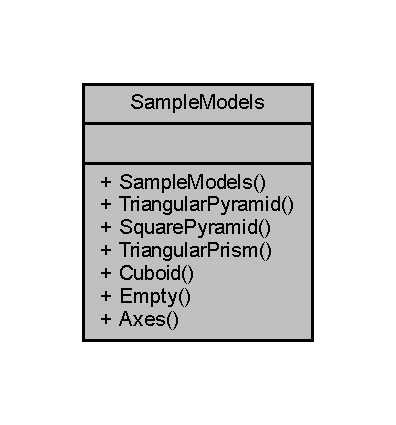
\includegraphics[width=190pt]{class_sample_models__coll__graph}
\end{center}
\end{figure}
\subsection*{Static Public Member Functions}
\begin{DoxyCompactItemize}
\item 
\mbox{\Hypertarget{class_sample_models_ac979fefcbc81571af56a2cf3c415497b}\label{class_sample_models_ac979fefcbc81571af56a2cf3c415497b}} 
static \mbox{\hyperlink{class_model}{Model}} $\ast$ {\bfseries Triangular\+Pyramid} (float side, float height)
\item 
\mbox{\Hypertarget{class_sample_models_a0a5afe183db2a5e7e59f825e6ac736e6}\label{class_sample_models_a0a5afe183db2a5e7e59f825e6ac736e6}} 
static \mbox{\hyperlink{class_model}{Model}} $\ast$ {\bfseries Square\+Pyramid} (float side, float height)
\item 
\mbox{\Hypertarget{class_sample_models_ad9be52995d798b78ad2c04c1b3c1f4e4}\label{class_sample_models_ad9be52995d798b78ad2c04c1b3c1f4e4}} 
static \mbox{\hyperlink{class_model}{Model}} $\ast$ {\bfseries Triangular\+Prism} (float side, float height)
\item 
\mbox{\Hypertarget{class_sample_models_a5e39e1ad1bcaec4b4ce617332e996caf}\label{class_sample_models_a5e39e1ad1bcaec4b4ce617332e996caf}} 
static \mbox{\hyperlink{class_model}{Model}} $\ast$ {\bfseries Cuboid} (float a, float b, float c)
\item 
\mbox{\Hypertarget{class_sample_models_a890001f4e859021afe59bd956245e2ad}\label{class_sample_models_a890001f4e859021afe59bd956245e2ad}} 
static \mbox{\hyperlink{class_model}{Model}} $\ast$ {\bfseries Empty} ()
\item 
\mbox{\Hypertarget{class_sample_models_a07f69bc5ff6c60078a642ba7e090bf6c}\label{class_sample_models_a07f69bc5ff6c60078a642ba7e090bf6c}} 
static \mbox{\hyperlink{class_model}{Model}} $\ast$ {\bfseries Axes} (float side)
\end{DoxyCompactItemize}


The documentation for this class was generated from the following files\+:\begin{DoxyCompactItemize}
\item 
src/samplemodels.\+h\item 
src/samplemodels.\+cpp\end{DoxyCompactItemize}

%--- End generated contents ---

% Index
\backmatter
\newpage
\phantomsection
\clearemptydoublepage
\addcontentsline{toc}{chapter}{Index}
\printindex

\end{document}
